\section{Empirical Findings}
\label{sec:findings}

This section reports what we found when we confronted the model with data. Each subsection states the question, describes the data and method, gives the result, and says what it does and does not show.

\subsection{Do investors with similar horizons hold similar portfolios?}
\label{sec:kappa}

\paragraph{Why this matters.} The central assumption of the model is that like trades with like. If real investors with similar horizons did not hold similar things, the clustering mechanism would have no counterpart in reality. This is the most direct empirical test of the model's foundation.

\paragraph{How we measure it.} In a given quarter, take every pair of managers $(i,j)$. For each pair compute two numbers.
\begin{enumerate}[leftmargin=*]
\item \emph{Portfolio similarity}: the cosine similarity of their portfolio weight vectors. Think of each portfolio as a list of weights over all securities. Cosine similarity is $1$ if two portfolios hold identical proportions of identical securities, and $0$ if they have no security in common.
\item \emph{Horizon closeness}: $\exp\!\big(-|\ln(\tau_i+1)-\ln(\tau_j+1)|\big)$. This equals $1$ for identical horizons and falls toward $0$ as horizons diverge. It is the same kernel the model uses to form links (Eq.~\eqref{eq:network} with $\kappa_h=1$).
\end{enumerate}
The \emph{horizon clustering score} $\hat\kappa_h$ for the quarter is the correlation, across all pairs, between these two numbers. A positive score means pairs with closer horizons hold more similar portfolios.

\begin{example}[Three pairs]
Using managers A, B, C from Table~\ref{tab:example}:
\begin{center}
\begin{tabular}{lrrr}
\toprule
Pair & Securities both hold & Portfolio similarity & Horizon closeness\\
\midrule
A and B & 346 & 0.079 & 0.222\\
A and C & 43 & 0.001 & 0.081\\
B and C & 195 & 0.132 & 0.363\\
\bottomrule
\end{tabular}
\end{center}
The pair with the closest horizons (B and C) also has the most similar portfolios, and the pair with the most distant horizons (A and C) has almost no overlap. Repeating this for every pair, roughly 3{,}600 to 5{,}700 pairs per quarter, gives the score.
\end{example}

\paragraph{Result.} The score is positive in all 50 quarters. Its average is $+0.158$ (standard deviation $0.043$ across quarters), with a smallest value of $0.051$ (Figure~\ref{fig:kappa}). Real investors with similar horizons do hold more similar portfolios. The effect is modest in size but remarkably consistent.

\begin{figure}[htbp]
\centering
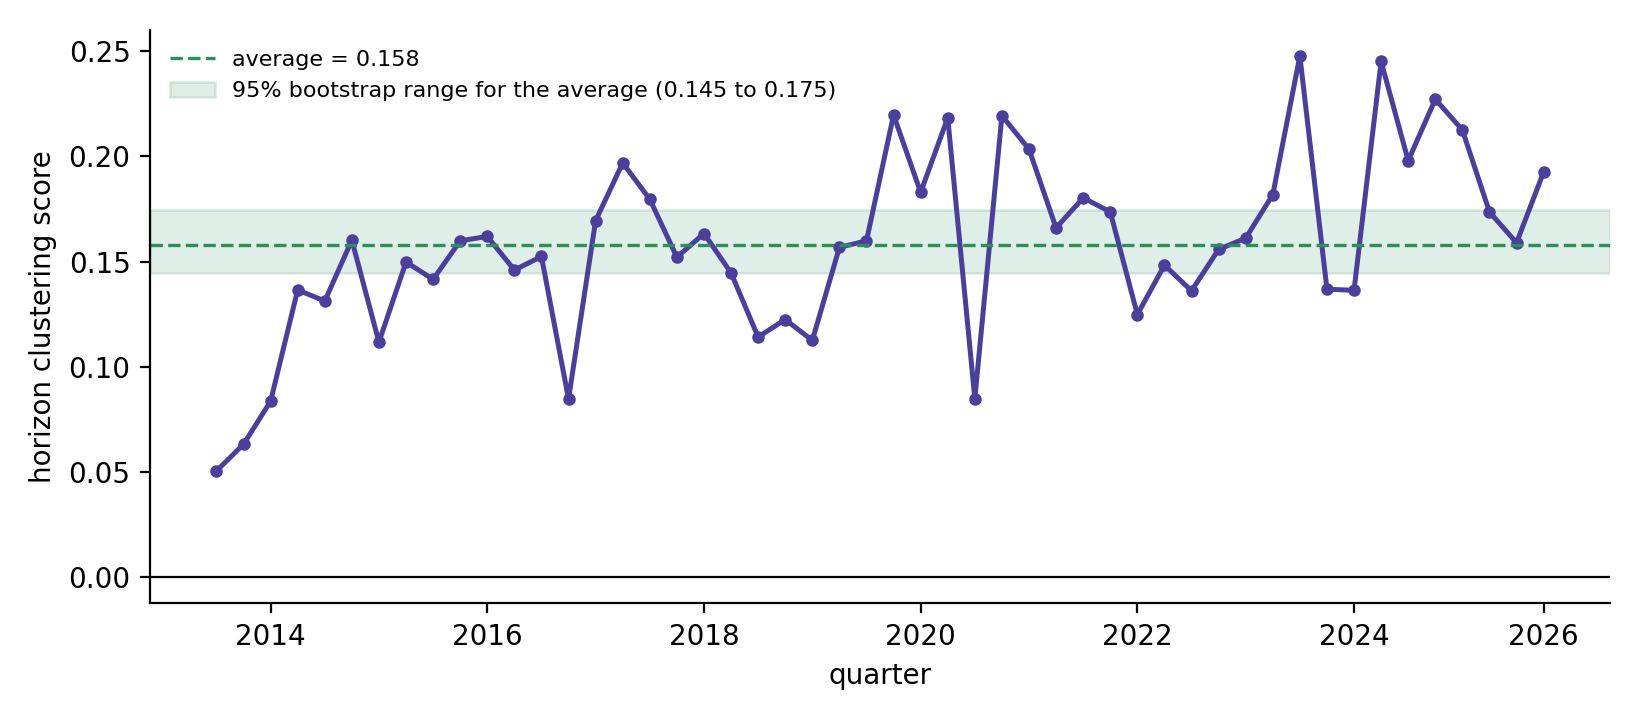
\includegraphics[width=0.85\linewidth]{kappa_series}
\caption{The horizon clustering score for each quarter, 2013 Q3 to 2026 Q1. The score is positive throughout. The shaded band is a 95\% range for the average obtained by resampling blocks of four quarters.}
\label{fig:kappa}
\end{figure}

\paragraph{How sure are we? Correcting for time dependence.} A simple test of whether the average differs from zero treats the 50 quarterly scores as independent, giving a $t$-statistic of $25.7$. But quarters are not independent: portfolios change slowly, so one quarter's score resembles the previous one. The correlation between one quarter's score and the next is $0.35$. A standard test confirms the pattern (the Ljung--Box test rejects ``no pattern'' at $p=0.012$ with one lag and $p=0.023$ with four, but not with eight lags, $p=0.10$).

The standard fix is the \emph{Newey--West correction}, which widens the uncertainty estimate to allow for each quarter resembling those nearby. It requires choosing a number of \emph{lags}, meaning how many neighbouring quarters are allowed to be related. A reviewer's natural question is how many lags are needed. Two standard formulas (Schwert's and Newey and West's 1994 rule) both give 3 lags. A third rule based on the series' own persistence gives 4. We also report longer lags up to 8 as a deliberately conservative check. Table~\ref{tab:lags} shows the result.

\begin{table}[htbp]
\centering
\caption{Newey--West $t$-statistic for the average clustering score being zero. A $t$ above about 2 is significant.}
\label{tab:lags}
\begin{tabular}{rrr}
\toprule
Lags & Standard error & $t$-statistic\\
\midrule
0 (no correction) & 0.0061 & 25.7\\
1 & 0.0071 & 22.1\\
2 & 0.0078 & 20.2\\
3 (chosen by two rules) & 0.0083 & 19.0\\
4 (chosen by third rule) & 0.0087 & 18.2\\
6 & 0.0093 & 17.1\\
8 & 0.0097 & 16.3\\
\bottomrule
\end{tabular}
\end{table}

More lags make the correction more cautious and the $t$-statistic falls, but it stays far above any threshold at every lag count. An earlier draft of our paper stated that the corrected statistic was about $15$ and referred to an effective sample size of 17; that figure came from a rough approximation and had never been computed. The effective sample size is in fact about 24 (computed as $50\times(1-0.35)/(1+0.35)$).

Two further checks agree. A \emph{block bootstrap}, which resamples blocks of four consecutive quarters to preserve their dependence, gives a 95\% range for the average of $0.145$ to $0.175$. A \emph{permutation test} addresses a separate problem: the roughly 5{,}000 pairs within a quarter are not independent of each other, since each manager appears in many pairs. We therefore reshuffle the horizons across managers 500 times within each quarter and ask how often a shuffled score is as large as the real one. The real score beats the shuffles at the 5\% level in 48 of 50 quarters (the exceptions are 2013 Q3 and 2013 Q4, the earliest quarters, with fewer reporting managers) and at the 1\% level in 47 of 50 (the third exception is 2016 Q4). This replaces an earlier claim that the score was highly significant in \emph{every} quarter, which did not survive the permutation test.

\paragraph{What the score does not show.} The score relates horizons to \emph{holdings} at one date, not to purchases or trades, so it does not show that investors \emph{buy} the same things. It also does not by itself tell us why horizon-similar managers hold similar stocks. And its relationship with the VIX is in the predicted direction but not significant ($r=+0.14$, $p=0.33$, 50 quarters).

\subsection{Is horizon diversity related to market volatility?}
\label{sec:drift}

\subsubsection{The original result}

Our original main empirical result was that horizon diversity (Eq.~\eqref{eq:tdi}) moves opposite to the VIX. Over 45 quarters, 2013 Q3 to 2024 Q3, the correlation is $r=-0.526$ ($p=0.0002$). Diversity was lowest in the Fed-tightening quarter 2022 Q4 ($1.02$) and fell sharply in the COVID-19 quarter 2020 Q1 ($1.55$); it was highest in calm 2019 Q2 ($1.99$). Figure~\ref{fig:tdi} shows the series.

\begin{figure}[htbp]
\centering
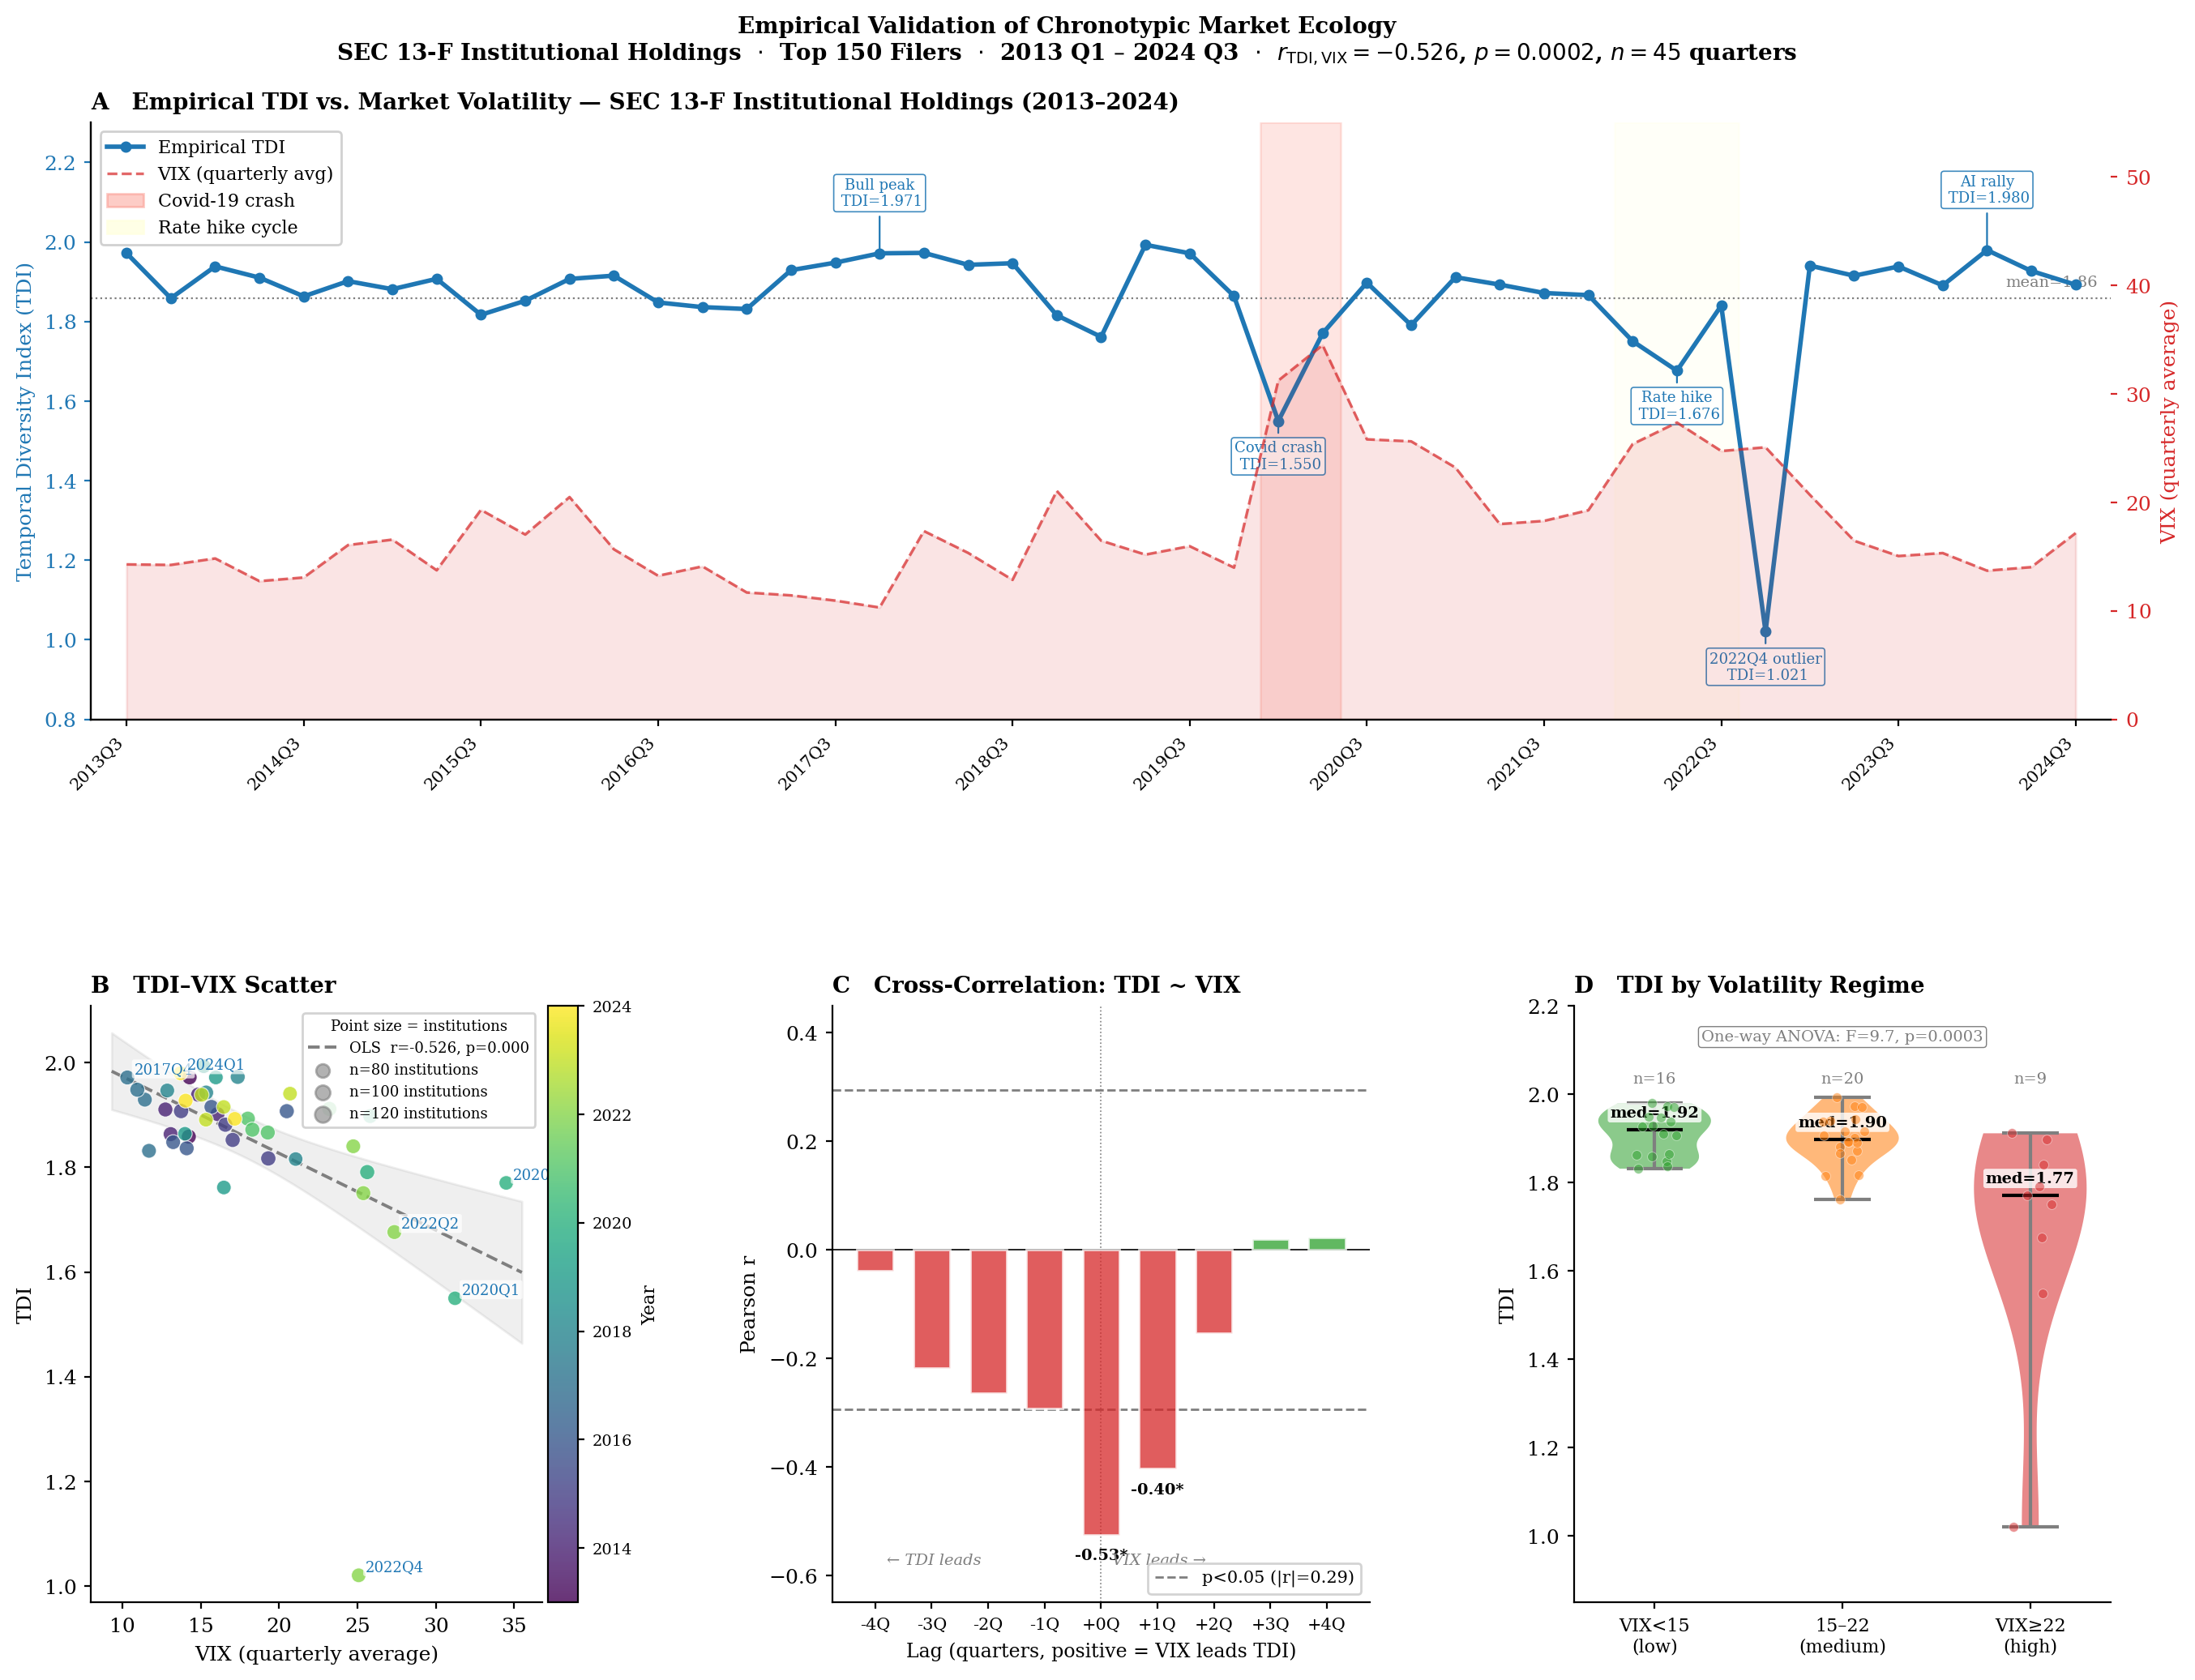
\includegraphics[width=\linewidth]{empirical_tdi_validation}
\caption{Original horizon diversity series (blue) and quarterly VIX (red dashed), 2013 Q3 to 2024 Q3.}
\label{fig:tdi}
\end{figure}

We also asked which series leads. A \emph{Granger test} asks whether last quarter's value of one series helps predict this quarter's value of another, beyond what the second series' own past predicts. It is a test of lead and lag, not proof of cause. In our original series, the VIX helps predict future diversity ($F=4.13$, $p=0.049$) but diversity does not help predict the VIX ($F=0.13$, $p=0.72$). Read naively, this says volatility compresses horizon diversity, the reverse of the direction in the model's story. A shock to diversity of one standard deviation reduces the VIX by about 1.9 points on impact in an impulse-response analysis, and an extended regression with policy-uncertainty and market-return controls gives an imprecise coefficient ($-3.80$, $p=0.18$). We reported these results while noting that the first was inconsistent with the direction the model emphasises.

\subsubsection{A problem we then found: price drift}

\begin{caution}[The central correction of this document]
Our measure of how often a manager trades turns out to be contaminated by price movements. When we remove that contamination, the link between horizon diversity and the VIX disappears.
\end{caution}

The turnover measure of Eq.~\eqref{eq:turnover} uses \emph{portfolio weights}, which are each holding's share of the portfolio's dollar value. But weights change whenever prices change, even if the manager does nothing at all.

\begin{example}[A manager who never trades]
A manager holds two stocks in equal amounts, so each has weight $50\%$. Over a quarter, stock A rises $10\%$ and stock B falls $10\%$, and the manager does nothing. The new weights are $1.10/2.00=55\%$ and $0.90/2.00=45\%$. The weight-based turnover is $\tfrac12(|0.55-0.50|+|0.45-0.50|)=5\%$, which implies a horizon of $63/0.05=1{,}260$ days. A true no-trade manager has an infinite horizon, so the measure has invented activity. In a volatile quarter, with bigger price moves, the invented turnover is bigger.
\end{example}

In volatile quarters prices move more, so weight-based turnover rises for everyone and horizons \emph{look} shorter, even with no change in behaviour. This would create a negative correlation between horizon diversity and the VIX with no behavioural content.

\paragraph{The test.} We rebuilt turnover from \emph{share counts} instead. For each security we use a single price (so that price changes cannot generate trades) and measure how many shares the manager actually bought or sold, as a fraction of the portfolio's value. We also repeat it after rebasing for stock splits, which change share counts without any trading. Everything else, including the managers, the bins and the formula, is unchanged.

Using our rebuilt data and the same VIX as the original (45 quarters), the correlation of horizon diversity with the VIX is:

\begin{table}[htbp]
\centering
\caption{Correlation of horizon diversity with the VIX under different turnover measures.}
\label{tab:drift}
\begin{tabular}{lrr}
\toprule
How turnover is measured & Correlation with VIX & 95\% range\\
\midrule
Change in portfolio weights (original method) & $-0.59$ & $-0.80$ to $-0.24$\\
Change in share counts & $-0.06$ & $-0.43$ to $+0.25$\\
Change in share counts, splits adjusted & $-0.10$ & $-0.49$ to $+0.27$\\
\bottomrule
\end{tabular}
\end{table}

The ranges come from a block bootstrap. The difference between the first two correlations is itself significant (95\% range $-0.92$ to $-0.13$). Figure~\ref{fig:drift} shows the two versions side by side. The weight-based measure tracks the VIX; the share-based measure does not.

\begin{figure}[htbp]
\centering
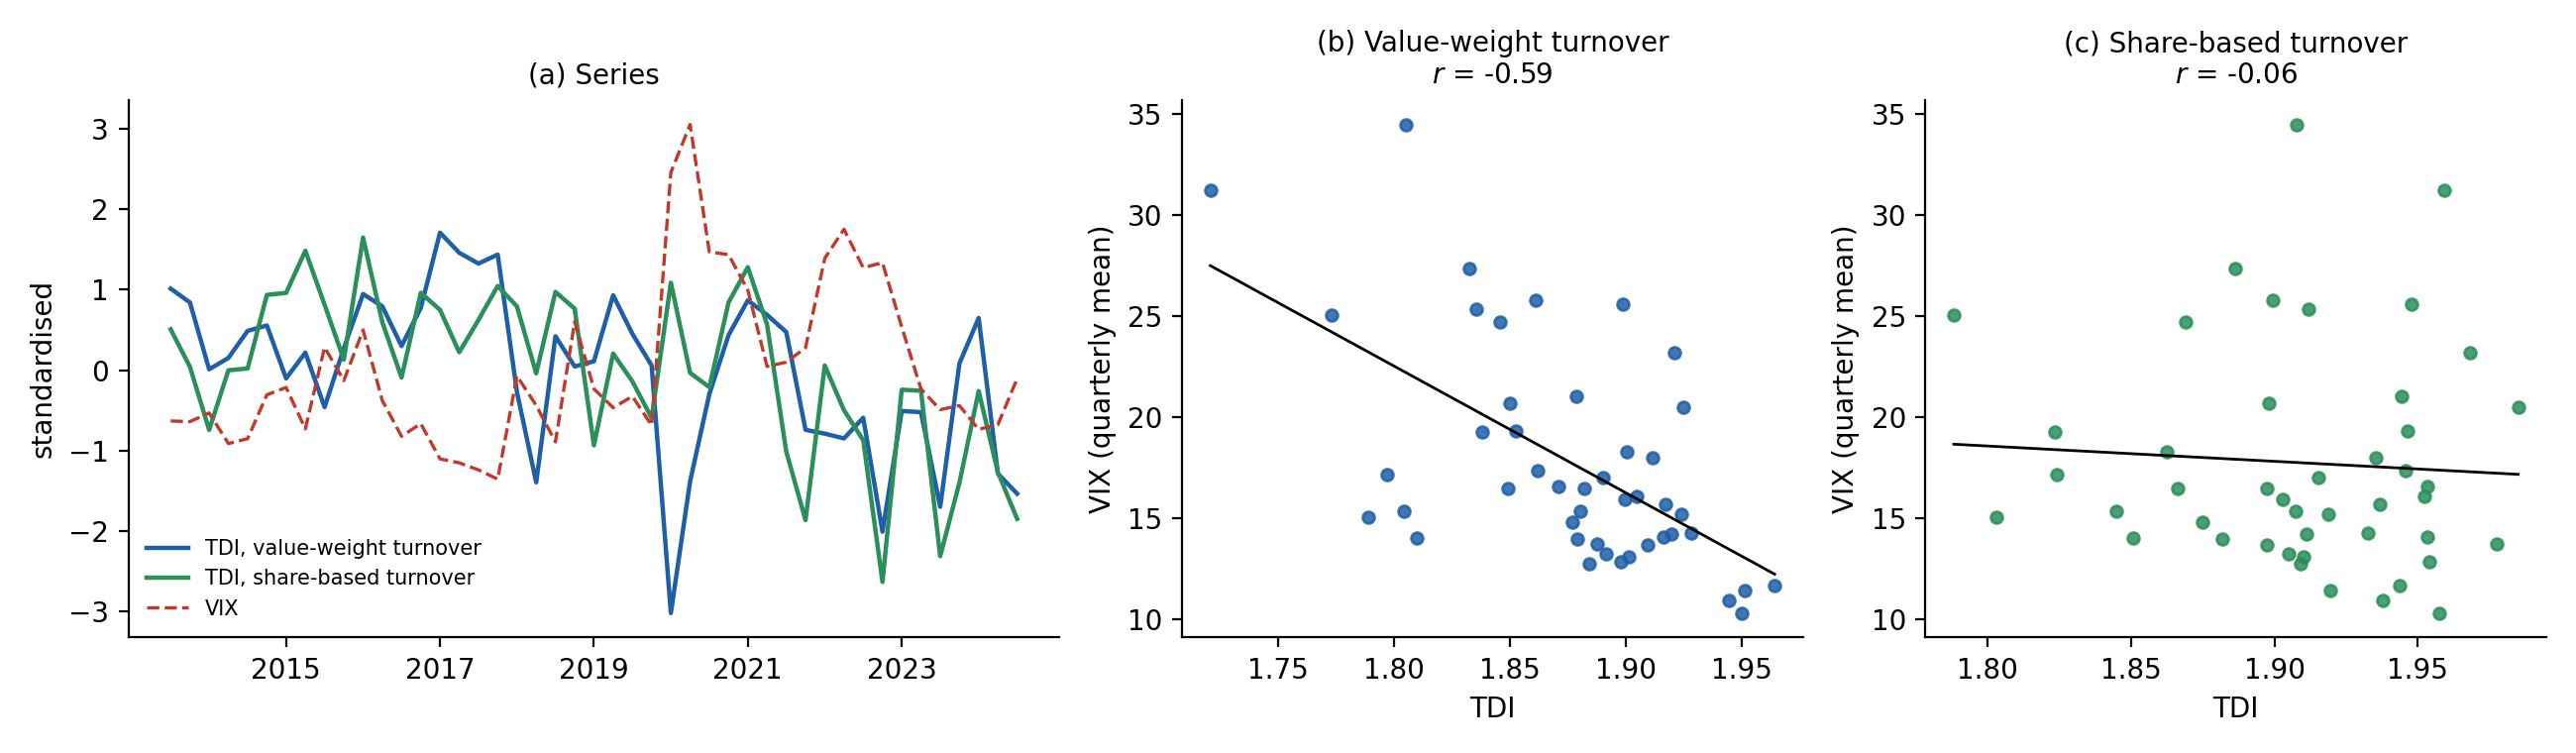
\includegraphics[width=\linewidth]{drift_check}
\caption{(a) Standardised horizon diversity built from weight-based turnover (blue) and share-based turnover (green), with the VIX (red dashed). (b) The weight-based measure falls when the VIX is high. (c) The share-based measure shows no relationship.}
\label{fig:drift}
\end{figure}

\paragraph{What this means.} Most of our original headline empirical result was a measurement effect. It should not be read as evidence that horizon diversity responds to, or influences, volatility. The Granger lead we found does not reproduce on the rebuilt series (VIX leads weight-based diversity at $p=0.73$ and share-based diversity at $p=0.21$, neither significant; with splits adjusted $p=0.08$), so we treat it as suggestive only.

\begin{caution}[A discrepancy we have not resolved]
Our rebuilt diversity series uses a somewhat different set of managers (114 to 135 per quarter versus 94 to 108 originally) and correlates only 0.50 with the original series. The largest gap is 2022 Q4, where the original series shows the lowest value in the sample ($1.02$) and the rebuilt one shows $1.77$. We have not identified the cause. For this reason, the comparison above is valid \emph{between turnover methods within the rebuilt data}, not as an exact copy of the original numbers.
\end{caution}

\subsubsection{Could there still be a real behavioural link?}

\citet{harrisraviv1993} argue that when investors disagree more, they trade more. Volatile times are times of greater disagreement, so a genuine behavioural reason for horizons to shorten when volatility rises is plausible. Our price-drift test shows that the \emph{accounting} channel explains most of what we measured. It does not rule out a real behavioural effect, only that our data cannot detect one. Separating the two would need trade-level data, or an event in which disagreement changes without price moving.

\subsection{Temporal liquidity: a result that was largely mechanical}
\label{sec:tl}

We built an empirical version of temporal liquidity from the S\&P~500 exchange-traded fund SPY. Each quarter we compute the volatility of quarterly returns over a rolling 4-quarter window and the first-order autocorrelation over a rolling 8-quarter window (using prices from 2011 so that every one of the 45 quarters is covered), and form TL by Eq.~\eqref{eq:tl}. The correlation of TL with the VIX is $-0.392$ ($p=0.008$, 45 quarters).

This looks like support for the model, but it is largely mechanical. Return volatility is \emph{inside} TL, in the denominator, so the logarithm of TL and minus the logarithm of volatility correlate at $0.90$. Realised return volatility correlates with the VIX at $0.76$, because the VIX tracks realised volatility. The other ingredient, return autocorrelation, which is the part carrying the model's mechanism, is unrelated to the VIX ($r=+0.04$, $p=0.81$). So the negative TL--VIX correlation tells us only that volatility is correlated with volatility. We do not count it as evidence for the mechanism. (An earlier draft reported this correlation on 36 quarters with an explanation about a burn-in period; the numbers are in fact from all 45 quarters, and that explanation was wrong.) TL is also uncorrelated with horizon diversity ($r=0.10$, $p=0.51$).

\subsection{Bond funds}
\label{sec:bonds}

\subsubsection{First attempt: average maturity}

Bond funds file holdings reports (Form N-PORT) that list every bond with its maturity date. For three large fund families (PIMCO, Vanguard, BlackRock), we computed each fund's \emph{weighted average maturity}, the dollar-weighted average of the remaining years to maturity, converted it to a horizon ($\text{years}\times252$ trading days), computed horizon diversity across funds each quarter, and correlated it with the MOVE index over 12 quarters, 2024 to 2026. The correlation was $-0.213$ ($p=0.51$), indistinguishable from zero.

We interpret this as an honest null result with an identifiable cause. Weighted average maturity reflects how a fund is \emph{built} (a short-term fund versus a long-term fund), set by its mandate and changing slowly, not how actively it \emph{trades}. The CME mechanism needs variation in active trading horizons, which this proxy does not capture.

\subsubsection{Second attempt: behavioural horizons by credit quality}

A reviewer suggested comparing bond funds with very different information environments, since in Treasury bonds essentially everyone has the same information whereas in high-yield (``junk'') corporate bonds some investors may know much more than others. We took seven Vanguard bond funds: short-, intermediate- and long-term Treasury; short-, intermediate- and long-term investment-grade corporate; and high-yield corporate. Each has 28 quarterly reports, giving 27 quarter-to-quarter changes.

To capture trading behaviour instead of fund design, we measure turnover from changes in the \emph{par amount} of each bond held, valued at a single price per bond so that price changes cannot generate trades, and we exclude bonds that simply matured. The behavioural horizon is then $63/\theta$ as before.

\begin{table}[htbp]
\centering
\caption{Seven Vanguard bond funds, 27 quarterly changes each. ``Link'' is the correlation across quarters, within each fund, with the MOVE index.}
\label{tab:bonds}
\small
\begin{tabular}{lrrrr}
\toprule
Fund & Average maturity (years) & Median trading horizon (days) & Link: maturity & Link: horizon\\
\midrule
Short-term Treasury & 3.75 & 146 & $-0.30$ & $+0.45$\\
Intermediate-term Treasury & 6.63 & 211 & $-0.54$ & $+0.44$\\
Long-term Treasury & 21.97 & 400 & $-0.40$ & $+0.30$\\
Short-term investment grade & 4.29 & 437 & $-0.64$ & $+0.47$\\
Intermediate-term investment grade & 8.40 & 363 & $-0.41$ & $+0.73$\\
Long-term investment grade & 22.84 & 765 & $-0.28$ & $+0.01$\\
High-yield corporate & 5.52 & 667 & $-0.31$ & $+0.36$\\
\bottomrule
\end{tabular}
\end{table}

Grouped by type, the median trading horizon is 218 days for Treasury funds, 454 days for investment-grade corporate funds and 667 days for high-yield funds. The funds with the most uncertain, dispersed information trade least often. Within each type, the behavioural horizon moves with the MOVE index with similar strength ($+0.38$ Treasury, $+0.33$ investment grade, $+0.36$ high yield): funds trade \emph{less} often when bond-market volatility is high. This is the opposite sign to the (now discounted) equity relationship in which horizons appeared to shorten when volatility rose, and it is consistent with a view that bond funds retreat in stressed periods. The average-maturity measure moves the other way (negative, as in the table), which fits the idea that maturity captures fund design and moves with the interest-rate environment rather than activity.

\begin{caution}[Interpret with care]
Each fund has only 27 observations and neighbouring quarters overlap. The pooled $p$-values within a type treat fund-quarters as independent although every fund in a given quarter shares one MOVE value, so we do not present them as formal tests. The results are descriptive.
\end{caution}

\subsection{A test on individual stocks}
\label{sec:stock}

\paragraph{Why move to stocks.} The aggregate relationship uses only 45 quarterly points, which gives little power and no way to control for other influences. Individual stocks give thousands of observations. The Fractal Market Hypothesis predicts that a stock owned by a narrow range of horizons should be more fragile than one owned by a wide mix. We can test that directly.

\paragraph{Measuring owner-horizon spread.} For a stock $s$ in a quarter, we take its owners among our panel of managers (requiring at least 10 owners). Let $w_{i,s}$ be manager $i$'s share of the panel's total dollar holding of $s$, and $\tau_i$ the manager's horizon from share-based turnover. The ownership-weighted average log horizon and spread are
\begin{equation}
\mu_s=\sum_i w_{i,s}\ln\tau_i,\qquad
\mathrm{DISP}_s=\sqrt{\sum_i w_{i,s}\,(\ln\tau_i-\mu_s)^2}.
\label{eq:disp}
\end{equation}
Low $\mathrm{DISP}_s$ means the stock's owners have similar horizons.

\paragraph{The question and the prediction.} Does low $\mathrm{DISP}_s$ in one quarter predict high volatility the next quarter? We fixed the prediction before looking at outcomes: the hypothesis predicts a \emph{negative} relationship (less spread, more volatility). The outcome is the log of the next quarter's realised volatility (standard deviation of daily returns, annualised). We also looked at the worst daily return and the skewness of returns as secondary outcomes.

\paragraph{Controls and methods.} Stocks differ in many ways, so we control for the owners' average horizon $\mu_s$ (which means we are asking about \emph{spread}, not about how short-term the owners are, which is the question of \citealt{cella2013}), the number of owners, how concentrated ownership is, the dollar amount held by our panel (a rough size proxy) and the stock's own current-quarter volatility (to guard against volatility simply persisting). All variables are standardised, so a coefficient reads as the change in next-quarter volatility, in standard deviations, per one standard deviation of owner spread.

We estimate in three ways. \emph{Fama--MacBeth} runs a separate cross-sectional regression each quarter and averages the coefficients, with the Newey--West correction on the time series of coefficients. \emph{Pooled with quarter fixed effects} compares stocks within the same quarter. \emph{Stock plus quarter fixed effects} compares each stock only with itself over time, removing anything permanent about a stock such as being large or being a blue chip; it is the most demanding test. As a falsification test (a \emph{placebo}), we randomly shuffle horizons across managers within each quarter, which should destroy any real relationship.

\paragraph{Data.} Starting from 44{,}573 distinct securities in the holdings, 2{,}449 had at least 10 owners in at least 30 quarters. After mapping to ticker symbols and keeping stocks with usable price histories, the sample is 63{,}261 stock-quarters covering 1{,}699 stocks over 48 quarters.

\begin{table}[htbp]
\centering
\caption{Effect of owner-horizon spread on next-quarter log volatility (standardised coefficients; more negative means that less spread goes with more volatility).}
\label{tab:stock}
\begin{tabular}{lrr}
\toprule
Method & Share-based horizons & Weight-based horizons\\
\midrule
Fama--MacBeth, average across quarters & $-0.046$ ($t=-6.2$) & $-0.044$ ($t=-8.0$)\\
Pooled, quarter fixed effects & $-0.017$ ($t=-4.1$) & $-0.009$ ($t=-2.3$)\\
Stock and quarter fixed effects & $-0.011$ ($t=-2.4$, $p=0.016$) & $-0.005$ ($p=0.26$)\\
Placebo (horizons shuffled) & $0.000$ ($t=0.01$) & not run\\
\bottomrule
\end{tabular}
\end{table}

\paragraph{Result.} Across stocks the relationship has the predicted sign and is statistically strong (Table~\ref{tab:stock}). But the effect shrinks as the comparison becomes more demanding. Within a single stock over time the coefficient is $-0.011$: a one-standard-deviation change in owner spread moves next-quarter volatility by about 1\% of a standard deviation. That is statistically detectable ($p=0.016$) but economically tiny, and with the weight-based horizons the within-stock effect is not significant. The placebo gives zero, as it should. The two secondary outcomes were not consistent: the worst daily return has the predicted sign in the Fama--MacBeth estimate but the opposite sign with fixed effects, and skewness shows no relationship.

\begin{caution}[Limits of the stock-level test]
(i) The price data are free data from Yahoo Finance, which \emph{drops delisted and acquired companies}, so the sample contains only survivors, which can bias volatility results. (ii) Only about 60\% of securities were matched to tickers, and current tickers can differ from historical ones. (iii) We have no true market capitalisation, so size is controlled only roughly, although the stock fixed effects remove permanent size differences. (iv) Our holdings cover 150 managers, not all institutions. The standard solution is the CRSP database, discussed in Section~\ref{sec:future}.
\end{caution}
